%!TEX root = ../main.tex

\section{Introduction}
\label{sec:intro}

State space models (SSMs) have achieved state-of-the-art sequence modeling performance in domains ranging from time series analysis~\citep{gu2022efficiently} to audio generation~\citep{goel2022s}.
However, they have yet to match the performance of Transformers on language modeling, often underperforming Transformers by multiple points in perplexity~\citep{gu2022efficiently}.
An natural question is whether this gap in performance is due to inherent inductive biases and capabilities in attention~\citep{edelman2022inductive,olsson2022context}, or whether it is a function of the significant organizational resources that have been spent training and tuning large attention-based language models~\citep{chowdhery2022palm,hoffmann2022training,zhang2022opt}, as well as specialized hardware support for attention, ranging from tensor cores~\citep{nvidia2017nvidia} to transformer chips~\citep{nvidia2022nvidia,kao2021optimized}.

We take first steps towards answering these questions in this paper.
First, we use synthetic language modeling tasks to show that there is an expressivity gap between SSMs and attention.
Using our insights, we design a new SSM layer that nearly matches attention in language modeling.
Second, we propose better hardware-aware algorithms for SSMs that allow them to take advantage of modern accelerators---and run faster than attention.

\begin{figure}
    \centering
    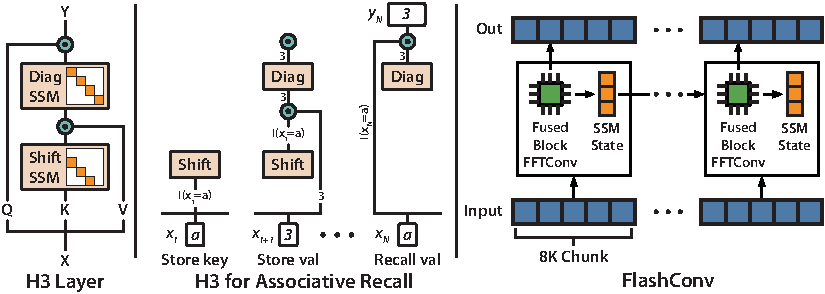
\includegraphics[width=\textwidth]{figs/banner_pdf.pdf}
    \caption{\label{fig:banner}
    Left: \hthree stacks two discrete SSMs with shift and diagonal matrices and uses multiplicative interactions between input projections and their outputs to model comparisons between points in a sequence.
    Middle: \hthree can perform associative recall---which is easy for attention, but not existing SSMs.
    Right: \fastfft uses a new state-passing algorithm over fused block FFTConv to increase hardware efficiency of SSMs, allowing \hthree to scale to billion-parameter models.
    }
    \vspace{-1.25em}
\end{figure}

\textbf{Understanding the Expressivity Gap.}
To understand the gap between SSMs and attention, we draw on synthetic language modeling tasks that have been proposed as a mechanistic basis for in-context learning in Transformers~\citep{olsson2022context}
These synthetic languages focus on the ability to manipulate text---recalling tokens from earlier time steps, or comparing tokens from different points in a sequence.
We find that existing SSMs struggle to model these synthetic languages.
To probe how important these skills are for language modeling, we propose \hthree (Hungry Hungry Hippo), a new SSM-based layer designed to solve these language modeling tasks.
\hthree stacks two SSMs, with multiplicative interactions between their outputs and input projections.
The SSMs allow \hthree to keep a log of tokens (to recall them later), while the multiplicative interactions allow for comparisons across the sequence.

\hthree matches attention on the synthetic languages and almost closes the gap with Transformers on language modeling---coming within \num{0.4} perplexity of Transformers on OpenWebText (compared to \num{3.4} ppl for existing SSMs---even those explicitly designed for language modeling~\citep{mehta2022long}).
Furthermore, a simple hybrid \hthree-attention model that retains two attention layers surprisingly \textit{outperforms} Transformers on OpenWebText by \num{1.0} perplexity.
To further evaluate \hthree on language modeling, we train 125M-, 355M-, 1.3B-, and 2.7B-parameter hybrid \hthree-attention language models on the Pile~\citep{gao2020pile}, using hyperparameters from GPT-3~\citep{brown2020language}.
These hybrid models outperform Transformer-based language models of the same size in perplexity, and match or outperform them on a majority of tasks in the SuperGLUE benchmark in zero- and few-shot learning.
Since the SSM layers in these hybrid models admit a recurrent view, they can also perform \num{2.4$\times$} faster inference than Transformers.
% These experiments moved to the Appendix
% Furthermore, \hthree maintains quality on non-text sequence modeling, matching the S4 model~\citep{gu2022efficiently} on raw speech classification and setting state-of-the-art performance on seizure classification over raw EEG signals.
% These results suggest that \hthree, or other SSM-attention hybrids, may be a promising direction for future language models or multimodal foundation models, especially with more resources towards finding optimal hyperparameters and training schedules for SSMs.

\textbf{Scaling SSMs.}
Next, we improve the efficiency of SSMs on modern hardware, to reduce the hardware barrier between attention and SSMs.
SSMs scale nearly linearly in sequence length instead of quadratically like attention, but still run slower on modern hardware due to poor hardware utilization.
To close this gap, we propose \fastfft, a hierarchical algorithm for computing SSMs, inspired by IO-Aware attention~\citep{dao2022flashattention}.
The technical challenge is that SSMs require a FFT-based convolution over the input sequence, which requires an FFT, pointwise multiply, and inverse FFT.
When implemented in cuFFT~\citep{cufft}, this operation incurs expensive GPU memory reads/writes, and cannot utilize the specialized matrix multiply units available on modern hardware\footnote{An A100 GPU has a maximum of 312 TFLOPs/s of FP16 with
tensor cores, but only 20 TFLOPs/s of FP32 (and 40 TFLOPs/s of FP16) without
tensor cores~\citep{nvidia2020nvidia}. This trend started with the V100 GPUs~\citep{nvidia2017nvidia} and has continued with the
H100 GPUs~\citep{nvidia2022nvidia}.}.
To use specialized matrix multiply units, we appeal to classical techniques that split the FFT into blocks and compute it using a series of matrix multiplications.
Combined with kernel fusion, this ``block'' FFT solution increases hardware efficiency, but only as long as the sequence length can fit into GPU SRAM (on-chip memory, analogous to L1 cache on the CPU)---up to sequence length 8K on modern A100.

To scale to sequences longer than 8K, we propose a \textit{state passing} algorithm (Figure~\ref{fig:banner} right), specialized to SSMs.
The key insight is that we can use the recurrent properties of SSMs to process the input in chunks---as long as we keep track of an additional state vector.
The state passing algorithm splits the input into the largest chunks that can fit into GPU SRAM, efficiently computes the FFT-based convolution using block FFT, and updates an intermediate state to start the next chunk.
Using this state-passing algorithm, \fastfft can scale SSMs to \textit{any} sequence length---even longer than can fit on GPU SRAM at once---while maintaining a \textit{near linear} compute complexity.
\fastfft sets state-of-the-art speed on long range arena using S4~\citep{gu2022efficiently}, outperforming Transformers by \num{5.8$\times$} and previous S4 models by \num{2$\times$}.
\fastfft trains \hthree\ \num{4-8$\times$} times faster than attention for long sequences, and is a critical component for scaling to billion-parameter models\footnote{Code for H3 is available at \url{https://github.com/HazyResearch/H3} }.

%%% Local Variables:
%%% mode: latex
%%% TeX-master: "../main"
%%% End:
